\documentclass[12pt]{article}
\usepackage{hyphsubst}
\usepackage[T2A]{fontenc}
\usepackage[utf8]{inputenc}
\usepackage[english,ukrainian,russian]{babel}
\usepackage{mathtools}
\usepackage{amsmath}
\usepackage{amsfonts}
\usepackage{graphicx}
\graphicspath{{pictures/}}
\DeclareGraphicsExtensions{.pdf,.png,.jpg}
\newcommand\aug{\fboxsep=-\fboxrule\!\!\!\fbox{\strut}\!\!\!}
\author{Аметов Имиль}
\title{Про то, что сделано}
\usepackage[thinlines]{easytable}
\usepackage[left=2cm,right=2cm,top=2cm,bottom=2cm,bindingoffset=0cm]{geometry}
\usepackage{indentfirst} % Для отступа первого абзаца
\begin{document}
\maketitle
\newpage
\tableofcontents
\newpage
\section{Метод Корад}

Развитие ядерной энергетики потребовало разработки неразрушающих методов определения загрязнения радионуклидами различных сред.

Первоначально для решения таких задач использовался метод с применением коллимированных сцинтилляционных спектрометрических детекторов на основе NaI(Tl) и одноканального спектроанализатора.

В начале 90-х были разработаны полноценные полевые спектрометры, с помощью которых были проведены иследования изменения сигналов в зависимости от глубины источника сигналов в почве с различными профилями. В результате исследований была разработана методика, позволяющая по измерениям скоростей счёта детектора в двух областях аппаратурного спектра (в фотопике --- 600-700 кэВ и в комптоновской области --- 400-600 кэВ) определять суммарную поверхностную активность загрязнения и примерную толщину загрязнённого слоя почвы. Этот вариант измерений был назван методом КОРАД (сокращение от <<КОллимированный РАДиометр>>).

Условная схема измерения по методу Корад показана на рис.\ref{fig:detector}.

\begin{figure}[h]
\center{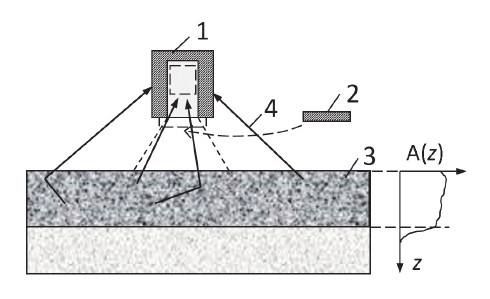
\includegraphics[scale=1]{detector.jpg}}
\caption{Принцип измерения коллимированным спектрометрическим детектором. \\ 1 --- спектрометрический детектор с защитой и коллиматором; 2 --- заглушка коллиматора; 3~---~загрязнённый слой с распределённой объёмной активностью ${}^{137}Cs$ в почве; 4 --- гамма-кванты нерассеянного и рассеянного излучения, регистрируемые детектором.}
\label{fig:detector}
\end{figure}

Для реализации такого метода нужно проводить два измерения --- основное без заглушки и дополнительное (фоновое) с заглушкой. В этом случае разностный спектр, в основном, формируется только теми гамма-квантами, которые прошли через коллиматор детектора, т.е. исключается влияние излучения, прошедшего через защиту.

Пример спектра для ${}^{137}$Cs полученный с помощью метода Корад показан на рис.\ref{fig:spectrum}. На этом рисунке представлено основное измерение, полученное при открытой заглушке коллиматора, фоновое измерение, полученное при закрытой заглушке коллиматора, разностный спектр, полученный с помощью вычитания из основного измерения фонового измерения и две энергетические области $\Delta E_1$ и $\Delta E_2$.

\begin{figure}[h]
\center{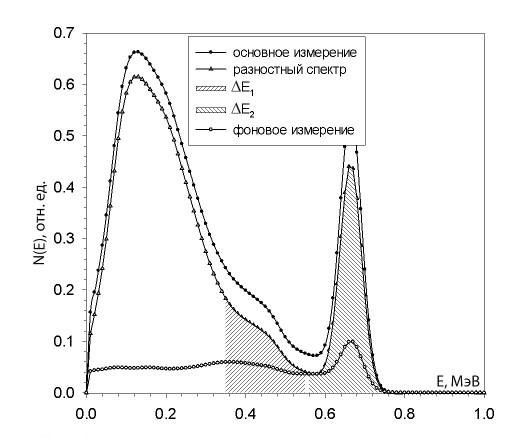
\includegraphics[scale=1]{spectrum.jpg}}
\caption{Аппаратурные спектры основного, фонового измерений и разностный спектр с указанием двух энергетических областей $\Delta E_1$ и $\Delta E_2$, используемых в методе Корад.}
\label{fig:spectrum}
\end{figure}

\section{Выбор библиотеки для создания искусственной нейронной сети}

  Для языка R существует большое количество самых разнообразных библиотек с реализацией тех или иных конструкторов нейронных сетей. Эти библиотеки различаются способами реализации нейронных сетей, предоставляемыми возможностями и предназначениями нейронных сетей. Из наиболее известных библиотек можно отметить такие библиотеки, как \verb|RSNNS|, \verb|nnet|, \verb|torch| и \verb|neuralnet|.

  Библиотека \verb|RSNNS| (Neural Networks using the Stuttgart Neural Network Simulator --- Нейронные сети, использующие Штутгардский симулятор нейронных сетей) представляет из себя набор нейросетей с различным назначением. В эту библиотеку входят нейронные сети для кластеризации объектов, для анализа временных рядов, для создания многослойных персептронных нейронных сетей и многого другого.

  Библиотека \verb|nnet| позволяет создавать и тренировать нейронные сети с одним скрытым слоем.

  Библиотека \verb|torch| представляет из себя интерфейс для каркаса машинного обучения \verb|PyTorch| с открытым исходным текстом программы. Каркас \verb|PyTorch| позволяет использовать вычислительные ресурсы графических процессоров для обучения и эксплуатации нейронных сетей.

  С помощью библиотеки \verb|neuralnet| возможно создавать, тренировать и использовать многослойные персептронные нейронные сети с гибкой архитектурой. Библиотека \verb|neuralnet| позволяет использовать как значения по-умолчанию, так и задавать свои значения. В возможностях библиотеки: гибко настраиваемое пороговое значение, максимально допустимое количество вычислительных операций, алгоритмы обратного распространения ошибки, задание пороговых функций. Поскольку в данной работе планировалось использовать персептрон, то было решено использовать именно библиотеку \verb|neuralnet| как наиболее подходящую для вычислений.

  \section{Особенности библиотеки neuralnet}

  Основной командой в библиотеке \verb|neuralnet| является команда \verb|neuralnet|. Синтаксис этой команды следующий:

\begin{verbatim}
neuralnet(formula, data, hidden = 1, threshold = 0.01, stepmax = 1e+05, rep = 1,
 act.fct = "logistic", linear.output = TRUE)
\end{verbatim}

  Аргумент \verb|formula| представляет символьное описание тренируемой модели.

  Пусть у нас есть кадр данных со следующими полями:

  \begin{tabular}{|c|c|c|c|c|}
    \hline
    \verb|x1| & \verb|x2| & ... & \verb|x20| & \verb|r| \\ \hline
  \end{tabular}

  И требуется натренировать нейросеть по входным аргументам \verb|x1|, \verb|x2|, ..., \verb|x20| и выходному значению \verb|r|. Все данные здесь вещественные числа. Тогда аргумент \verb|formula| будет представлен как

\begin{verbatim}
r ~ x1 + x2 + ... + x20
\end{verbatim}

  Аргумент \verb|data| представляет название того кадра данных, по которому проводится тренировка нейросети.

  Аргумент \verb|hidden| представляет вектор с описанием внутренних слоёв нейронной сети. Пример: ``\verb|hidden = 1|'' обозначает, что будет использована нейросеть, с одним внутренним слоем, состоящим из одного-единственного нейрона, ``\verb|hidden = c(10,9,5)|'' обозначает, что в нейронной сети будет три внутренних последовательно связанных слоя из десяти, девяти и пяти нейронов соответственно.

  Аргумент \verb|threshold| --- это числовое значение, определяющее пороговое значение для ошибки, по достижению которого останавливается процесс тренировки нейронной сети. По-умолчанию, значение \verb|threshold| равно 0.01.

  Аргумент \verb|stepmax| указывает максимальное количество шагов для тренировки нейронной сети. Если в процессе тренировки сети будет превышено это число шагов, то тренировка прекратится с предупреждением об ошибке. По-умолчанию, число шагов 100000.

  Аргумент \verb|rep = 1| определяет раз будет запущен процесс тренировки. По-умолчанию, тренировка запускается только один раз.

  Аргумент \verb|act.fct| указывает функцию активации нейрона. В самой библиотеке \verb|neuralnet| описано две функции: \verb|"logistic"| (логистическая) и \verb|"tanh"| (гиперболический тангенс).

  Логистическая функция --- это функция вида $P(t) = \dfrac {1} {1+e^{-t}}$.
  Гиперболический тангенс~---~функция вида $P(t) = \dfrac {2} {1 + e^{-2t}} - 1$.

  Аргумент ``\verb|linear.output = TRUE|'' обозначает, что результ работы выходного нейрона будет линейным, а ``\verb|linear.output = FALSE| обозначает необходимость применения функции активации из \verb|act.fct| для выходного нейрона.

  Другой важной функцией является функция \verb|predict.nn|. Эта функция используется после того как будет натренирована нейронная сеть командой \verb|neuralnet|. Назначение функции \verb|predict.nn| в эксплуатации нейросети с уже подобранными под задачу весовыми коэффициентами.

  Синтаксис этой функции:

\begin{verbatim}
predict (object, newdata)
\end{verbatim}

  Аргумент \verb|object| --- объект, представляющий нейронную сеть, аргумент \verb|newdata| --- матрица или кадр данных из которых следует извлечь данные для вычислений.

  \section{Описание программы}
  
\begin{enumerate}

\item {Создание тренировочного набора данных}

  Для создания тренировочного набора данных используется команда

  \verb|trainingSet <- mkDataFrame (5000)|

  то есть создаётся кадр данных под названием \verb|trainingSet|, генерирует этот кадр данных функция под названием \verb|mkDataFrame|. Эта функция принимает в качестве аргумента целочисленное положительное число, обозначающие количество записей, которые нужно сгенерировать. Отсюда вызов команды \verb|mkDataFrame (5000)| порождает кадр данных, который можно представить в виде следующей таблицы:

  \begin{tabular}{|c|c|c|c|c|c|}
    \hline
    $x_1$ & $x_2$ & ... & $x_{20}$ & $r$ & depth \\ \hline
    0 & 0 & ... & 0 & 1.0 & 10 \\ \hline
    0 & 0 & ... & 0 & 1.0 & 10 \\ \hline
    0 & 0 & ... & 0 & 1.0 & 10 \\ \hline
    0.005 & 0.004 & ... & $4.39 \cdot 10^{-8}$ & 0.7 & 7 \\ \hline
  \end{tabular}

  Вообще говоря, содержимое кадра данных, возвращаемого функцией \verb|mkDataFrame| каждый раз будет новым и будет отличаться от предыдущего вызова.

  Значения полей $x_1$, $x_2$, $...$, $x_{20}$ являются значениями бинов, поле $r$ --- это нормализованное значение толщины незаражённого поверхностного слоя. При этом для $r$ максимальное значение равно 1 (соответствует значению поля \emph{depth} равному 10), а минимальное значение равно 0 (соответствует значению поля \emph{depth} равному 0). Поле \emph{depth} --- это толщина незаражённого слоя, измеряемая в половинах длин свободного пробега.

  Текст функции \verb|mkDataFrame| следующий:

\begin{verbatim}
mkDataFrame <- function (n) {
    tmpDF <- data.frame ()
    for (i in (seq (1, n))) {
        tmpDF <- rbind (tmpDF, (mk20BinsRnd ()))
    }
    names (tmpDF) [1:22] <- c ("x1", "x2", "x3", "x4", "x5", "x6", "x7", "x8",
                               "x9", "x10", "x11", "x12", "x13", "x14", "x15",
                               "x16", "x17", "x18", "x19", "x20", "r", "depth")
    return (tmpDF)
}
\end{verbatim}

  В строке \verb|tmpDF <- data.frame ()| происходит создание пустого кадра данных.

  Наполнением кадра данных занимается цикл

\begin{verbatim}
    for (i in (seq (1, n))) {
        tmpDF <- rbind (tmpDF, (mk20BinsRnd ()))
    }
\end{verbatim}

  Создание очередной записи происходит в строке \\ \verb|tmpDF <- rbind (tmpDF, (mk20BinsRnd ()))|. Созданием записи занимается функция с названием \verb|mk20BinsRnd|, со следующим текстом:

\begin{verbatim}
1. mk20BinsRnd <- function () {
2.    myKoefs <- mlps ()
3.    mySpectrum <- superposition (myKoefs)
4.    bins <- getBins (20, mySpectrum [300:730])
5.    bins <- c (bins, (firstNullsCount (myKoefs)) / 10)
6.    bins <- c (bins, (firstNullsCount (myKoefs)))
7.    return (bins)
}
\end{verbatim}

  В этой функции создаётся набор \verb|myKoefs| (2-я строка) из десяти коэффициентов, эти коэффициенты используются для создания спектра \verb|mySpectrum| с помощью функции \verb|superposition (myKoefs)| (3-я строка), из этого спектра формируются 20 бинов с отбором значений на отрезке $[300;730]$ (4-я строка). К бинам добавляется нормализованная толщина незаражённого слоя (5-я строка) и ненормализованная толщина незаражённого слоя (6-я строка). В 7-й строке происходит возврат бинов.

  Функция \verb|mlps| определена следующим образом:

\begin{verbatim}
mlps <- function () {
    return (mkCoefs())
}
\end{verbatim}

  То есть, происходит вызов функции \verb|mkCoefs| с телом

\begin{verbatim}
1. mkCoefs <- function() {
2.    a1 <- sample (0:10, 1)
3.    a2 <- sample (-5:10, 1)
4.    a3 <- sample (1:3, 1)
5.    rf <- function (x) {
6.        a1 / (exp (abs (((x - a2) / a3)^3)))
7.    }
8.    return (round (rf (1:10)))
9. }
\end{verbatim}

  В функции \verb|mkCoefs| создаются три случайные значения $a_1$ (на отрезке $[0; 10]$), $a_2$ (на отрезке $[-5; 10]$ и $a_3$ (на отрезке $[1;3]$). В строках 5-7 происходит создание функции-замыкания \verb|rf|, которую математически можно описать как

  $$f(x) = a_1 e^{- \left | {\frac {x - a_2} {a_3}} \right |^3}.$$

  В строке 8 эта функция применяется на вектор-последовательность (1, 2, 3, 4, 5, 6, 7, 8, 9, 10) и полученная последовательность возвращается из функции.

  Тело функции \verb|superposition| задано таким образом:

\begin{verbatim}
1. superposition <- function (koeffs) {
2.     result <- rm01 * koeffs [1] + rm02 * koeffs [2] +
3.         rm03 * koeffs [3] + rm04 * koeffs [4] +
4.         rm05 * koeffs [5] + rm06 * koeffs [6] +
5.         rm07 * koeffs [7] + rm08 * koeffs [8] +
6.         rm09 * koeffs [9] + rm10 * koeffs [10]
7.     result <- unlist (map (result, noise))
8.     return (result)
}
\end{verbatim}

  Эта функция получает аргумент-вектор из десяти коэффициентов \verb|koeffs|, умножает эти коэффициенты на векторы \verb|rm01|, \verb|rm02| и так далее, до вектора \verb|rm10| (эти векторы получены с помощью программы <<Корад>>). В 7-й строке добавляется шум. И возвращает сумму этих векторов. Полученный вектор представляет собой спектр.

  Функция добавления шума реализована таким образом:

\begin{verbatim}
1. noise <- function (x) {
2.     x <- x + 0.1E-05 * (2 * runif(1) - 1)
3.     if (x < 0) x <- 0
4.     return (x)
}
\end{verbatim}

  Здесь аргументом является вектор \verb|x|, во 2-й строке к нему добавляется случайное значение из отрезка $[-10^{-6}, 10^{-6}]$. В 3-й строке значения вектора, оказавшиеся меньше нуля исправляются на нуль. Четвёртая строка возвращает зашумленный вектор из функции.
  
  Вернёмся к функции \verb|mk20BinsRnd|, а именно к 4-й строке \newline \verb|bins <- getBins (20, mySpectrum [300:730])|. Здесь происходит вызов функции \\ \verb|getBins|. Функция \verb|getBins| служит для разделения значений спектра с индексами от 300 до 730 на 20 бинов.

  Текст функции \verb|getBins|:

\begin{verbatim}
1. getBins <- function (n, vctr) {
2.     tmp <- c ()
3.     len <- length (vctr)
4.     group <- len / n
5.     for (i in (seq (1, len, by = group))) {
6.         tmp <- c (tmp, mean (vctr [i : (i + group - 1)]))
7.     }
8.     return (tmp)
}
\end{verbatim}

  В строках 5 и 6 функции \verb|mk20BinsRnd| формируются нормализованная и ненормализованная толщина незаражённого вещества. Под этой толщей находится источник радиоактивного излучения.

\item{Тренировка нейросети}

  Перед тренировкой нейросети нужно загрузить библиотеку командой

  \verb|library (neuralnet)|

  Нейросеть тренируется следующей командой:

\begin{verbatim}
nn <- neuralnet (r ~ x1 + x2 + x3 + x4 + x5 + x6 + 
                 x7 + x8 + x9 + x10 + x11 + x12 + 
                 x13 + x14 + x15 + x16 + x17 + x18 + 
                 x19 + x20, data = trainingSet, 
                 act.fct = "logistic", linear.output = F)
\end{verbatim}

\item{Создание тестового набора данных}

  Тестовый набор данных формируется аналогично учебному набору, но с числом записей равным тысяче.

\begin{verbatim}
testSet <- mkDataFrame (1000)
\end{verbatim}

\item{Создание кадра данных с нормализованными значениями толщины незаражённого вещества (первая колонка) и со значениями толщины незаражённого вещества вычисленное нейросетью (вторая колонка).}

\begin{verbatim}
comparison.dataframe <- cbind (testSet [, 21], 
                               compute (nn, 
                                        testSet [, 1:20])$net.result)
\end{verbatim}

\item{Сохранение кадра данных \verb|comparison.dataframe| в файл \verb|output.txt|.}

  Для сохранения кадра данных \verb|comparison.dataframe| в файл \verb|output.txt|. Применяется команда

\begin{verbatim}
write.table (comparison.dataframe, file = "output.txt", 
             append = FALSE, sep = "\t", row.names = FALSE, 
             col.names = FALSE)
\end{verbatim}

\item{Формирование картинки на основе данных из файла \verb|output.txt|.}

  Для формирования картинки была применена программа \verb|gnuplot| с такой программой:

\begin{verbatim}
gnuplot -e "set terminal png size 10240,480; set style fill pattern; 
            set style histogram clustered; set style data histogram; 
            set xrange [-1:1000]; set output \"graph.png\"; 
            plot \"output.txt\" u 1 t \"Оригинал\", 
                           \"\" u 2 t \"Предсказание\""
\end{verbatim}

  Исходные данные обозначены незаштрихованным столбцом, а значения, вычисленные нейросетью --- заштрихованным столбцом.
\end{enumerate}

\section{Описание нейросети для определения толщины загрязнённого слоя}

Для создания тренировочного набора данных использовалась команда

\begin{verbatim}
trainingSetThickness <- mkDataFrameThickness (5000)
\end{verbatim}

Эта команда создаёт кадр данных под названием \verb|trainingSetThickness|, который состоит из 5000 записей и 102-х столбцов. Первыми идут столбцы под названием \verb|x1|, \verb|x2|, ..., \verb|x100|. В этих столбцах находится содержимое 100 бинов. Как показала практика, двадцать бинов оказалось недостаточно для тренировки нейросети для определения толщины загрязнённого слоя. Поэтому пришлось применить разбиение входных данных на большее количество бинов. В данном случае --- сто бинов.

Сто первая и сто вторая колонки содержат толщину загрязнённого слоя в нормализованном (от 0 до 1) и в ненормализованном (от 0 до 10) виде.

Текст функции \verb|mkDataFrameThickness|:

\begin{verbatim}
mkDataFrameThickness <- function (n) {
    tmpDF <- data.frame ()
    for (i in (seq (1, n))) {
        tmpDF <- rbind (tmpDF, (mk100BinsRndThick ()))
    }
    names (tmpDF) [1:102] <- c ("x1", "x2", "x3", "x4", "x5", "x6", "x7", "x8",
                               "x9", "x10", "x11", "x12", "x13", "x14", "x15",
                               "x16", "x17", "x18", "x19", "x20", "x21", "x22",
                               "x23", "x24", "x25", "x26", "x27", "x28", "x29",
                               "x30", "x31", "x32", "x33", "x34", "x35", "x36",
                               "x37", "x38", "x39", "x40", "x41", "x42", "x43",
                               "x44", "x45", "x46", "x47", "x48", "x49", "x50",
                               "x51", "x52", "x53", "x54", "x55", "x56", "x57",
                               "x58", "x59", "x60", "x61", "x62", "x63", "x64",
                               "x65", "x66", "x67", "x68", "x69", "x70", "x71",
                               "x72", "x73", "x74", "x75", "x76", "x77", "x78",
                               "x79", "x80", "x81", "x82", "x83", "x84", "x85",
                               "x86", "x87", "x88", "x89", "x90", "x91", "x92",
                               "x93", "x94", "x95", "x96", "x97", "x98", "x99",
                               "x100", "r", "thickness")
    return (tmpDF)
}
\end{verbatim}

Эта функция практически ничем не отличается по внутреннему строению от функции \verb|mkDataFrame|. Отличия заключаются лишь в использовании функции \verb|mk100BinsRndThick|, и в добавлении имён для новых столбцов.

Текст функции \verb|mk100BinsRndThick|:

\begin{verbatim}
mk100BinsRndThick <- function () {
    myKoefs <- mlps ()
    materialThickness <- length (myKoefs [myKoefs > 0])
    mySpectrum <- superposition (myKoefs)
    bins <- getBins (100, mySpectrum [300:730])
    bins <- c (bins, materialThickness / 10)
    bins <- c (bins, materialThickness)
    return (bins)
}
\end{verbatim}

Толщина загрязнённого слоя определяется с помощью команды

\begin{verbatim}
materialThickness <- length (myKoefs [myKoefs > 0])
\end{verbatim}

Разделение спектра на сто бинов выполняет команда

\begin{verbatim}
bins <- getBins (100, mySpectrum [300:730])
\end{verbatim}

Создание и тренировка нейросети выполнялась с помощью команды

\begin{verbatim}
nnThickness <- neuralnet (r ~ x1 + x2 + x3 + x4 + x5 + x6 + x7 + x8 + x9 + x10 + 
                          x11 + x12 + x13 + x14 + x15 + x16 + x17 + x18 + x19 +
                          x20 + x21 + x22 + x23 + x24 + x25 + x26 + x27 + x28 +
                          x29 + x30 + x31 + x32 + x33 + x34 + x35 + x36 + x37 +
                          x38 + x39 + x40 + x41 + x42 + x43 + x44 + x45 + x46 +
                          x47 + x48 + x49 + x50 + x51 + x52 + x53 + x54 + x55 +
                          x56 + x57 + x58 + x59 + x60 + x61 + x62 + x63 + x64 +
                          x65 + x66 + x67 + x68 + x69 + x70 + x71 + x72 + x73 +
                          x74 + x75 + x76 + x77 + x78 + x79 + x80 + x81 + x82 +
                          x83 + x84 + x85 + x86 + x87 + x88 + x89 + x90 + x91 +
                          x92 + x93 + x94 + x95 + x96 + x97 + x98 + x99 + x100,
                          data = trainingSetThickness, hidden = 4, 
                          act.fct = "logistic", linear.output = F)
\end{verbatim}

Тестовый набор данных \verb|testThickness| был создан с помощью команды

\begin{verbatim}
testThickness <- mkDataFrameThickness (1000)
\end{verbatim}

Вычисление нейросетью \verb|nnThickness| толщины загрязнённого слоя были сохранены в список \verb|resultsThickness|:

\begin{verbatim}
resultsThickness <- predict (nnThickness, testThickness [, 1:100])
\end{verbatim}

\section{Статистический анализ погрешности работы нейросети}

Абсолютной погрешностью приближённого числа $a$ называется величина $\Delta_a$, удовлетворяющая неравенству

$$\Delta_a \ge |A - a|.$$

Абсолютные погрешности предсказания были вычислены с помощью команды

\begin{verbatim}
errors <- abs (testSet[21] - results)
\end{verbatim}

С помощью этой команды создаётся объект \verb|errors| с типом ``список'', в который помещён модуль разности между контрольной глубиной залегания радиоактивного материала \verb|testSet[21]| и предсказанным результатом \verb|results|.

Для тестового набора данных c шумом \verb|testClear| было вычислены абсолютные погрешности:

\begin{verbatim}
errorsClear <- abs (resultsClear - testClear[21])
\end{verbatim}

Для тестового набора без шума максимальная абсолютная погрешность вычислена с помощью команды

\begin{verbatim}
max (errors)
\end{verbatim}

И составила 0.07455158. Или, с учётом нормализации (деления показания глубины на десять) составляет примерно

$$0.07455158 \cdot 10 = 0.7455158 \approx 1.$$

То есть, предсказания нейросети ошибаются на 1 половину длины свободного пробега.

Для тестового набора с шумом максимальная абсолютная погрешность составила

\begin{verbatim}
> max (errorsClear)
[1] 0.07770665
\end{verbatim}

С учётом нормализации это также приблизительно одна половина свободного пробега.


Выборочное среднее абсолютной погрешности можно вычислить с помощью команды

\begin{verbatim}
mean (unlist (errors))
\end{verbatim}

Получен результат 0.01049212 без шума и 0.01444896 с шумом.

Найдём несмещённую дисперсию. Несмещённая дисперсия $S^2$ вычисляется по формуле

$$S^2 = \dfrac {1} {n-1} \sum_{i=1}^{n}(x_i - X).$$

где $n$ --- количество элементов в выборке, $x_i$ --- $i$-й элемент выборки, $X$ --- выборочное среднее из выборки.

Для нахождения несмещённой дисперсии в языке R есть функция \verb|var|. Воспользуемся ею:

\begin{verbatim}
var (unlist (errors))
\end{verbatim}

был получен результат 0.0002085357 без шума и 0.0003160496 с шумом.

\section{Статистический анализ погрешности nnThickness}

Абсолютные погрешности результатов вычислений нейросети \verb|nnThickness| для тестового набора данных \verb|testThickness| были сохранены в список \verb|errorsThickness|:

\begin{verbatim}
errorsThickness <- abs (resultsThickness - testThickness[101])
\end{verbatim}

Максимальная абсолютная погрешность при вычислении толщины заражённого слоя без шума составила 0.3159411, а с шумом 0.305306. Или около трёх половин длин свободного пробега. Средняя абсолютная погрешность без шума составила 0.06462503, с шумом 0.06079966. Или примерно одна половина длины свободного пробега. Несмещённая дисперсия для данных без шума составила 0.004126353, а с шумом 0.003706332.


\end{document}